% This is "sig-alternate.tex" V2.0 May 2012
% This file should be compiled with V2.5 of "sig-alternate.cls" May 2012
%
% This example file demonstrates the use of the 'sig-alternate.cls'
% V2.5 LaTeX2e document class file. It is for those submitting
% articles to ACM Conference Proceedings WHO DO NOT WISH TO
% STRICTLY ADHERE TO THE SIGS (PUBS-BOARD-ENDORSED) STYLE.
% The 'sig-alternate.cls' file will produce a similar-looking,
% albeit, 'tighter' paper resulting in, invariably, fewer pages.
%
% ----------------------------------------------------------------------------------------------------------------
% This .tex file (and associated .cls V2.5) produces:
%       1) The Permission Statement
%       2) The Conference (location) Info information
%       3) The Copyright Line with ACM data
%       4) NO page numbers
%
% as against the acm_proc_article-sp.cls file which
% DOES NOT produce 1) thru' 3) above.
%
% Using 'sig-alternate.cls' you have control, however, from within
% the source .tex file, over both the CopyrightYear
% (defaulted to 200X) and the ACM Copyright Data
% (defaulted to X-XXXXX-XX-X/XX/XX).
% e.g.
% \CopyrightYear{2007} will cause 2007 to appear in the copyright line.
% \crdata{0-12345-67-8/90/12} will cause 0-12345-67-8/90/12 to appear in the copyright line.
%
% ---------------------------------------------------------------------------------------------------------------
% This .tex source is an example which *does* use
% the .bib file (from which the .bbl file % is produced).
% REMEMBER HOWEVER: After having produced the .bbl file,
% and prior to final submission, you *NEED* to 'insert'
% your .bbl file into your source .tex file so as to provide
% ONE 'self-contained' source file.
%
% ================= IF YOU HAVE QUESTIONS =======================
% Questions regarding the SIGS styles, SIGS policies and
% procedures, Conferences etc. should be sent to
% Adrienne Griscti (griscti@acm.org)
%
% Technical questions _only_ to
% Gerald Murray (murray@hq.acm.org)
% ===============================================================
%
% For tracking purposes - this is V2.0 - May 2012

\documentclass{sig-alternate}
\graphicspath{{figures/}}
\newfont{\mycrnotice}{ptmr8t at 7pt}
\newfont{\myconfname}{ptmri8t at 7pt}
\let\crnotice\mycrnotice%
\let\confname\myconfname%

\permission{Permission to make digital or hard copies of all or part of this work for personal or classroom use is granted without fee provided that copies are not made or distributed for profit or commercial advantage and that copies bear this notice and the full citation on the first page. Copyrights for components of this work owned by others than ACM must be honored. Abstracting with credit is permitted. To copy otherwise, or republish, to post on servers or to redistribute to lists, requires prior specific permission and/or a fee. Request permissions from permissions@acm.org.}
\conferenceinfo{BCB'16,}{October 2--5, 2016, Seattle, WA, USA.}
\copyrightetc{Copyright 2016 ACM \the\acmcopyr}
\crdata{978-1-4503-4225-4/16/10\ ...\$15.00.\\
http://dx.doi.org/10.1145/2975167.2985844}

\clubpenalty=10000
\widowpenalty = 10000

\begin{document}

\title{Automated Verification of Phenotypes using PubMed}
%\subtitle{
%\titlenote{A full version of this paper is available as
%\textit{Author's Guide to Preparing ACM SIG Proceedings Using
%\LaTeX$2_\epsilon$\ and BibTeX} at
%\texttt{www.acm.org/eaddress.htm}}}
%
% You need the command \numberofauthors to handle the 'placement
% and alignment' of the authors beneath the title.
%
% For aesthetic reasons, we recommend 'three authors at a time'
% i.e. three 'name/affiliation blocks' be placed beneath the title.
%
% NOTE: You are NOT restricted in how many 'rows' of
% "name/affiliations" may appear. We just ask that you restrict
% the number of 'columns' to three.
%
% Because of the available 'opening page real-estate'
% we ask you to refrain from putting more than six authors
% (two rows with three columns) beneath the article title.
% More than six makes the first-page appear very cluttered indeed.
%
% Use the \alignauthor commands to handle the names
% and affiliations for an 'aesthetic maximum' of six authors.
% Add names, affiliations, addresses for
% the seventh etc. author(s) as the argument for the
% \additionalauthors command.
% These 'additional authors' will be output/set for you
% without further effort on your part as the last section in
% the body of your article BEFORE References or any Appendices.

\numberofauthors{5} %  in this sample file, there are a *total*
% of EIGHT authors. SIX appear on the 'first-page' (for formatting
% reasons) and the remaining two appear in the \additionalauthors section.
%
\author{
% You can go ahead and credit any number of authors here,
% e.g. one 'row of three' or two rows (consisting of one row of three
% and a second row of one, two or three).
%
% The command \alignauthor (no curly braces needed) should
% precede each author name, affiliation/snail-mail address and
% e-mail address. Additionally, tag each line of
% affiliation/address with \affaddr, and tag the
% e-mail address with \email.
%
% 1st. author
\alignauthor
Ryan Bridges\\
       \affaddr{Epic Systems}\\
       \affaddr{Verona, WI 53593}\\
       \email{rybridges90@gmail.com}
% 2nd. author
\alignauthor
Jette Henderson\\
       \affaddr{The University of Texas at Austin}\\
       \affaddr{Austin, TX 78712}\\
       \email{jette@ices.utexas.edu}
% 3rd. author
\alignauthor Joyce C Ho \\
       \affaddr{Emory University}\\
       \affaddr{Atlanta, GA 30322}\\
       \email{joyce.c.ho@emory.edu}
\and  % use '\and' if you need 'another row' of author names
% 4th. author
\alignauthor Byron C. Wallace \\
       \affaddr{Northeastern University}\\
       \affaddr{Boston, MA, 02115}\\
       \email{byron@ccs.neu.edu}
% 5th. author
\alignauthor Joydeep Ghosh\\
       \affaddr{The University of Texas at Austin}\\
       \affaddr{Austin, TX 78712}\\
       \email{jghosh@utexas.edu}
}
% There's nothing stopping you putting the seventh, eighth, etc.
% author on the opening page (as the 'third row') but we ask,
% for aesthetic reasons that you place these 'additional authors'
% in the \additional authors block, viz.

% Just remember to make sure that the TOTAL number of authors
% is the number that will appear on the first page PLUS the
% number that will appear in the \additionalauthors section.

\maketitle
\begin{abstract}
In the realm of data driven clinical research, medical concepts, or phenotypes, are used to serve as indicators for patient clusters of interest. Often, studies will use groups of algorithmically generated phenotypes (feature groups) to predict the occurrence of heart disease, diabetes, and other conditions. 
When these groups are algorithmically generated, the most common method of verification is manual human annotation, which can be time consuming and sometimes inconsistent.
In this paper, we propose a supervision-free method of verification that uses co-occurrence in PubMed articles to determine clinical significance.
We demonstrate the efficacy of the method by 1) applying it to phenotypes generated through automatic machine learning methods and 2) showing it separates randomly generated groups of phenotypes from curated groups of known, clinical phenotypes. 
\end{abstract}

% A category with the (minimum) three required fields
\category{H.3.3}{Information Search and Retrieval}{Information filtering}
%A category including the fourth, optional field follows...
\category{I.2.7}{Natural Language Processing}{Text analysis}
\category{J.3}{Life and Medical Sciences}{Health}
\terms{Phenotype verification, Pubmed, co-occurrence analysis}

\section{Introduction}

Computational phenotyping is the practice of mapping the raw information contained in Electronic Health Records (EHRs) into sets of clinically relevant features, or phenotypes.
Clinicians can use the EHR-based phenotypes to identify patients with specific characteristics or conditions of interest.
Phenotypes also enable cohort identification to target patients for screening tests and interventions, support surveillance of infectious diseases, and aid in the conduct of pragmatic clinical trials and comparative effectiveness research \cite{Collaboratory:MR-x2zyZ}.
An example is the type 2 diabetes mellitus phenotype (shown in Figure \ref{fig:t2d-pheno}) \cite{kho_use_2012}.
The flowchart depicts a series of characteristics that must be present in a patient's EHR for that patient to be identified as a type 2 diabetes case patient.

\begin{figure} [t]
\centering
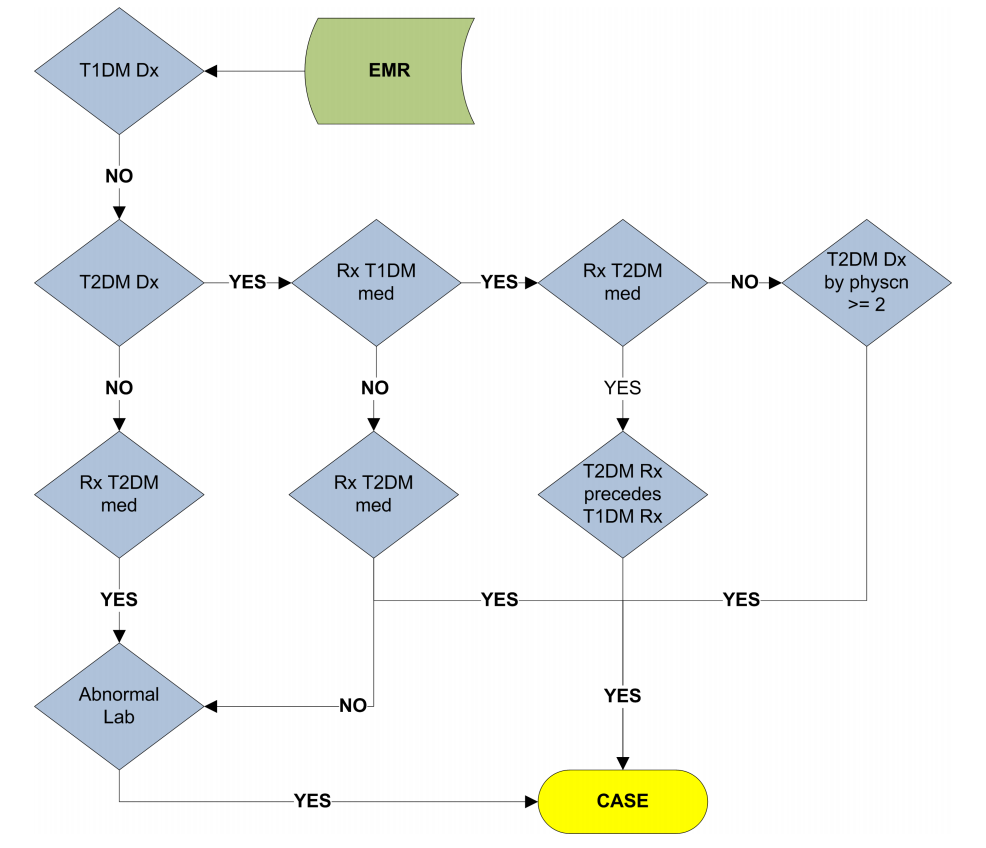
\includegraphics[width=\linewidth]{t2d-pheno.png}
\caption{Type 2 diabetes phenotype from the Phenotype Knowledgebase \cite{kho_use_2012}, Source: https://phekb.org/phenotype/type-2-diabetes-mellitus}
\label{fig:t2d-pheno}
\end{figure}

Constructing phenotypes can be a manual, iterative, and labor-intensive process requiring domain expertise \cite{carroll2011naive,chen2013applying,hripcsak2013next}. 
Recent efforts have focused on machine learning developed methods to automatically generate candidate computational phenotypes in a high-throughput, unsupervised manner \cite{Ho:2014jc,Ho:2014da, hu2015scalable, wang2015rubik,Yu:2015fj}.
%Figure (see Figure \ref{fig:pheno-example} for candidate phenotypes generated by automatic methods).
%Figure \ref{fig:decomp-example} illustrates the conceptual process of a high--throughput, automatic phenotype generation process \cite{hripcsak2013next} to aid the discovery of knowledge.
However, domain experts are still required to annotate these candidate phenotypes to verify the clinical significance, and several issues can arise during the annotation process beyond time--consumption.
First, domain experts may disagree on the clinical relevance of a candidate phenotype. 
%For example, annotators disagreed on the clinical significance of the phenotype generated by the method detailed in \cite{Ho:2014da}'s method shown in Figure \ref{tab:pheno-example}. 
Second, unsupervised methods may generate phenotypes that are unfamiliar to annotators, so they may incorrectly judge a phenotype as clinically insignificant when it is not.
Additionally, given the diverse and different clusters of patients grouped by these methods, annotators may feel the objective or the phenotypes themselves are vague or undefined.
Thus, there is a need to develop an automated, data--driven process to serve as an unbiased means of validation, leveraging all the medical expertise that has been collected to date.
%\begin{figure} [t]
%\centering
%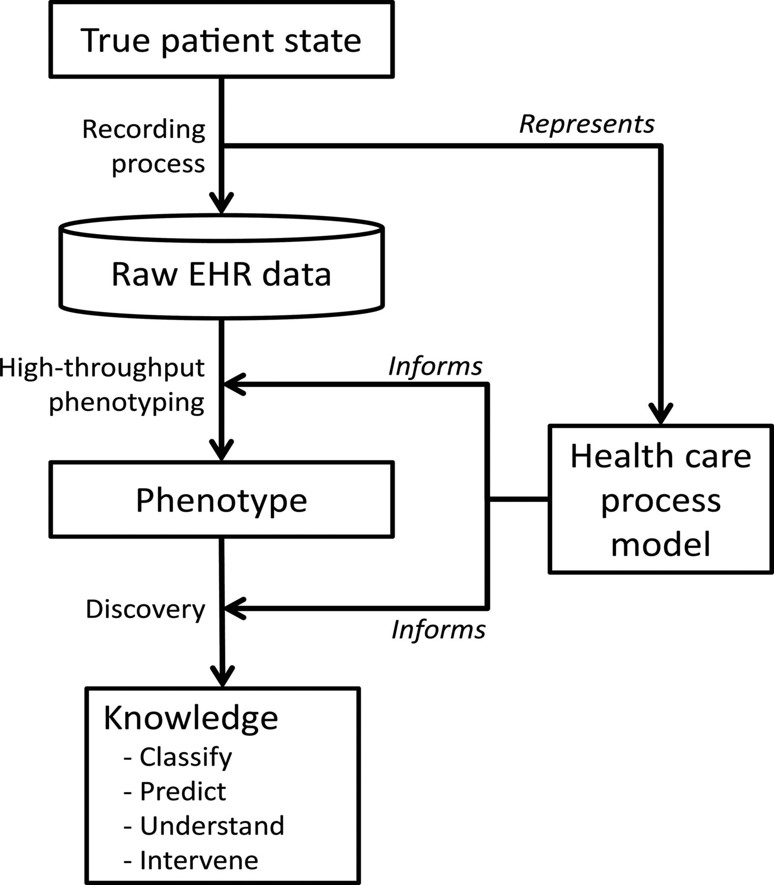
\includegraphics[width=0.75\linewidth]{example-phenotype-process.jpg}
%\caption{Overview of high-throughput phenotype generation process \cite{kho_use_2012}.}
%\label{fig:decomp-example}
%\end{figure}


%\begin{figure*} [t]
%\centering
%\includegraphics[width=\linewidth]{marble-lambda-pheno.png}
%\caption{Examples of candidates phenotypes generated through a high-throughput automatic process}
%\label{fig:pheno-example}
%\end{figure*}


%As data driven clinical research is used more in decisions for business and medicine, consistent phenotype verification will become increasingly important.
In this paper, we present an automated framework that can provide third-party verifcation to facilitate and improve the annotation process and accuracy.
%In this paper, we present a framework that automates the process of annotating candidate phenotypes, and has the potential to facilitate the annotation process and improve annotation accuracy.
Our method records co--occurrences of phenotypic terms in PubMed\footnote{http://www.ncbi.nlm.nih.gov/PubMed}, a publicly available repository for medical literature that contains over 40GB of medical literature from over 6000 journals. 
From this data, we use lift, a metric that summarizes if two or more items co--occur more often than average while accounting for the commonality of the item, to determine clinical relevance.
%From co-occurrence data in PubMed, we calculate lift of phenotypes (lift is a metric summarizing if two or more items co-occur more often than on average, taking into account if an item is more common than another).
%High lift between two or more phenotypic items suggests they are clinically related. 
We analyze the lift patterns of 80 phenotypes produced by several of the high--throughput methods described above and demonstrate the correlation between lift with the significance as judged by domain experts.
%We analyze the lift patterns amongst phenotypes produced by the high-throughput methods described above.
We also illustrate the upper and lower bounds of the lift metric by comparing phenotypes generated randomly to those curated to represent known medical concepts.
%We also compare phenotypes generated randomly to those curated to represent known medical concepts.
%In this way, we show upper and lower bounds for significance as measured by lift, and demonstrate the correlation between significance measured by lift with significance as judged by domain experts.
We demonstrate the method is agnostic to the algorithm that generated the phenotypes by showing it can effectively determine the validity of candidate phenotypes produced by two different high-throughput algorithms, as well as curated phenotypes. We note however, that if an algorithm itself uses PubMed to generate phenotypes, this method of verification should not be used.
%While this method could be used to replace human annotation, we present it more as a tool for the annotation process.
%In addition to corroborating human annotation, automatic labeling can be used to facilitate the annotation process. Previous work (\cite{neveol2011semi}) has shown that annotators produce better annotations in less time when starting from pre-annotated results from automatic tools.

%\begin{table}
%\begin{center}
%\begin{tabular}{l}
%\toprule
%\color{blue}Hypertension \\
%\color{blue}Osteoarthrosis and allied disorders \\
%\color{blue}Urinary tract infection \\
%\color{red}Analgesics\\
%\bottomrule
%\end{tabular}
%\end{center}
%\caption{Example of a candidate phenotype where annotators disagree on ``clinical significance". Blue entries represent the patient's diagnoses, red entries are medications.}
%\label{tab:pheno-example}
%\end{table}


\section{Related Work}
While many researchers have used PubMed to explore and discover issues in biology, medicine, and health informatics, few have used PubMeb as a validation tool.
One such study by Boland et al. mined EHR records for patients who had disease-specific codes and then compared the association between birth month and the disease to a group of control patients who did not have the disease codes present in their EHRs \cite{boland2015birth}. 
They validated their results against papers queried from PubMed that had disease and birth month as topics.
Neveol  et al. did not use Pubmed as a validation tool but they did use it as a tool to generate candidate annotations for PubMed queries and then measured the inter-annotator agreement as well as annotation time between sets of queries with and without the candidate annotations \cite{neveol2011semi}. 
While they were annotating PubMed in order to understand PubMed users' needs, their work shows that annotating tools can not only speed up annotating time, but increase inter-annotator agreement.
However, annotating before annotators can examine the text can have the effect of biasing annotators, so it should be used carefully.

More commonly, researchers PubMed as an exploratory tool.
%Multiple software packages like LitInspector \cite{frisch2009litinspector} and PubMed.mineR as well as python packages like Pymedtermino\footnote{\url{http://pythonhosted.org/PyMedTermino/}} and Biopython\footnote{\url{http://biopython.org/}} have been developed to help researchers extract and visualize PubMed.
Jensen et al. provide a thorough overview of how PubMed can be harnessed for information extraction and entity recognition \cite{jensen2006literature}.
Amongst the two methods they discuss for information extraction, natural language processing and co--occurrence analysis, co--occurrence is more prevalent due to its straightforward implementation and the intuitive interpretation of the results.
%Among the two methods they discuss for information extraction, natural language processing and co--occurrence analysis, we focus on co--occurrence because of its straightforward implementation and the intuitive interpretation of the results (i.e., two terms that appear together more frequently are associated).
While co--occurrence analysis does not give information about the type of relationship or any causal information, work done on bias towards publishing positive results allows for the assumption that when two phrases occur together the relationship exists \cite{dickersin1990existence,easterbrook1991publication,stern1997publication}.
Researchers have applied co-occurrence strategies to generate phenotypes. 
Some have used Pubmed to study links between diseases \cite{rajpal2014mining}, which can be thought of as phenotype discovery, and to explore relationships between phenotypes and genotypes \cite{pletscher2015diseases}.
Having generated phenotypes through machine learning techniques, our work focuses on using co-occurrence analysis of Pubmed as a validation tool for annotations.

%Raijpal et al. perform frequency analyses on PubMed abstracts in order to 1) predict emerging trends in genes and the diseases to which they are related and 2) explore the possible link between two diseases, psoriasis and obesity \cite{rajpal2014mining}. 
%This type of exploration can be thought of as phenotype discovery.

%Co--occurrence analysis of PubMed has also been used to explore relationships between phenotypes and genotypes.
%Pletscher-Frankild et al. perform co--occurrence analysis on the abstracts along with genetic data and evidence from other studies to discover disease-gene associations \cite{pletscher2015diseases}.
%They apply a scheme that takes into account co--occurrence within an abstract and within a sentence, and then convert the co--occurrence scores into Z-scores, which corrects for abstracts of different lengths.
%Adding another layer of complexity to the co-occurrence, \cite{von2015data} queried MEDLINE for a set of diseases, to construct disease by genes vectors where a vector element is zero or replaced by the number of times the disease and gene co--occur in articles. 
%This approach, called second order co--occurrence, is meant to model the idea even though diseases may no occur together frequently, they belong to a cluster of diseases that co--occur frequently overall, which they ascertain through thresholding the cosine similarity of the disease vectors.
%
%PubMed has also been used as a resource for generating annotations.

%Our work uses co-occurence methods to validate results generated through high-throughput methods.
%While we apply co-occurence to perform validation of high-throughput phenotyping methods, this approach could be applied to other types of experiment results.

\begin{figure*} [t]
\centering
\includegraphics[width=\linewidth]{Flowchart_Features_revised.png}
\caption{Feature extraction for Phenotypic Items}
\label{fig:feature-extract}
\end{figure*}

\section{Method}
Annotators are often clinicians volunteering their time, and may or may not have computational backgrounds or annotation experience.
Furthermore, medical perspectives can be drastically different amongst annotators as they are impacted by factors such as their medical expertise, patient population, and medical education (medical school and residency).
%Furthermore, medical expertise is likely to be different amongst annotators, shaping their medical perspectives. 
In addition to these reasons, the vague and subjective nature of the annotation task can result in low inter--rater agreement amongst the different clinicians, with one high--throughput phenotyping method reporting an inter--rater agreement of 0.81 \cite{wang2015rubik}.
%These reasons, along with the fact that the annotation task may be interpreted differently amongst annotators introduce the fact that annotators often disagree about labels.
%Our automated method produces labels that capture any common causation amongst phenotypic items in a corpus of medical literature.
We propose to leverage the $26+$ million biomedical literature citations found in PubMed as an objective third--party annotator by developing an automated method to capture co-occurrence of phenotypic items within the clinical narratives described throughout PubMed.
Our framework utilizes the inherent publication biases associated with medical literature to observe that if a concept pairing is clinically significant, several papers will make mention of these concepts together in such a large and diverse corpus.
%In our experiment, we use PubMed Central as our corpus in order to utilize the wide variety of disciplines represented in PubMed. \jette{cite specifically what PubMed and Medline are}
%We rely on the assumption that if a concept pairing is clinically significant, several papers will make mention of these concepts together in such a large and diverse corpus. 
This provides a reasonable objective baseline for determining significance that can be used as corroboration for existing annotation or as a tool to assist annotation efforts.

Although the idea is conceptually simple, there are several challenges that our automated framework must address.
The representation of each element of the phenotype is important as it can drastically impact the number of articles returned during the PubMed query.
Second, the co--occurrence search needs to account for encoding, form/tense, incorrect spellings, and also regularization.
Finally, the co--occurrence metric should reflect the number of items contained in the phenotype elements as well as the commonality of the item itself in the PubMed literature.
Thus, our automated verification process consists of several steps:
\begin{enumerate}
\item Feature (n-gram) generation from phenotypes
\item Counting co-occurrence in PubMed articles
\item Calculating and normalizing feature lifts within a particular group to determine significance
\end{enumerate}
Figures \ref{fig:feature-extract} and \ref{fig:sig-calc} show the process for a phenotype from the feature generation to the calculation of the clinical significance.
%Figures 3 and 4 summarize how features are generated for each phenotypic item and how clincal significance is determined.

\begin{figure*} [t]
\centering
\includegraphics[scale=.6]{Flowchart_ToLift.png}
\caption{Significance calculation for phenotypic items}
\label{fig:sig-calc}
\end{figure*}

%Figure \ref{fig:feature-extract} shows
%Our co--occurrence uses the lift 

%Because lift, the co-occurrence metric we use, normalizes for frequency mentioned in the corpus, the method can capture the significance of common concepts as well as well as rare concepts that co-occur more frequently than average. 

\subsection{Feature Extraction}
Since medical terms can have multiple synonyms and representations across different articles, our framework first generates a suitable list of synonyms and related concepts for each element in the phenotype (each phenotypic item).
The leftmost box of Figure \ref{fig:feature-extract} displays an example of a candidate phenotype, which was generated by an automatic method, that could be presented to the annotators.
In this example, the term ``heart failure" can also be referred to in various articles using other terms such ``myocardial failure", ``congestive heart disease", or may be even be referred to in the context of more general terms such as ``cardiovascular health".
Thus, the appropriate terms must be used so that heart failure as a concept may be discovered in a PubMed article reasonably often when it is being mentioned (recall); however, the terms may not be so general as to produce many false positives (precision).
%Each item in the phenotype has to be suitably represented so that it may be discovered in a PubMed article reasonably often when it is being mentioned (recall), but not produce many false positives (precision).
To produce a representation that has high recall and high precision, we first generate a large set of possible representative n-grams, and then filter all the candidate n-grams down to the most relevant n-grams (the filtration process is discussed in the next section).
%Often times, the phenotype elements themselves have been aggregated using an existing hierarchy (e.g., PheWAS groupings for ICD-9 diagnosis codes, ATC codes for medications, etc.). 

A na\"{\i}ve approach is to use the item as it appears rather than to perform the candidate generation and filtration process.
However, this can yield low recall as the text is often too specific or not phrased naturally. 
For example, note the phenotypic item ``calcium channel blocking agents" in the phenotype in Figure \ref{fig:feature-extract}. 
When searching through text, it may be more appropriate to shorten the phrase to ``calcium channel blockers" or even alternatively use the phrase  ``hypertension medications." 

Likewise, using a collection of individual words (unigrams) to represent phenotypes yields high recall, but low precision, as it is difficult to filter out enough of the words that lack specificity, but are important in some cases (e.g. ``disease" or ``results").
``Calcium", ``channel", ``blocking", and ``agents" will obviously find all occurrences of ``calcium channel blocking agents," but will also capture mentions having little to do with the subject, resulting in low precision.

%\begin{table}
%{\small
%\begin{tabular}{l}
%\hline
%Alzheimer's disease, unspecified \\
%Malignant carcinoid tumor of the bronchus and lung \\
%Stress fracture, hip, unspecified, sequela \\
%Other disorders of kidney and ureter in diseases classified elsewhere \\
%Vitamins and minerals \\
%Angiotensin-converting enzyme inhibitors \\
%\hline
%\end{tabular}
%}
%\caption{Phenotype group in the ``clinically significant" ground truth set}
%\label{tab:clinical-significant-phenotype}
%\end{table}

In order to achieve high recall, a phenotypic item must be recognized when a conceptually equivalent or similar term is present and capture situations when an entirely dissimilar string is used to represent the same item  (e.g. ``heart attack" and ``myocardial infarction").
In order to recognize such ``aliases," we utilized several medical ontologies to collect a set of closely related concepts and synonyms to a given phenotypic item.
One of the most complete and commonly used ontologies is the ``Systemized Nomenclature of Medicine - Clinical Terms" (SNOMED-CT) ontology \cite{Wasserman2003}. The first order connections on the SNOMED-CT ontology graph for a concept provided a reasonable number of aliases that we could then filter.
We supplemented SNOMED-CT with two other common ontologies, ICD--10 and the NCBI MeSH terms.
During implementation, we extracted the SNOMED-CT and ICD--10 ontologies with a python library called Pymedtermino.\footnote{http://pythonhosted.org/PyMedTermino/}
Biopython,\footnote{http://biopython.org/} a tool which also provides an interface to the Entrez tools, provided access to the MeSH terms.
We queried the Pymedtermino and Entrez APIs to collect aliases from these three ontologies, and then placed the related terms from each ontology into a (potentially large) list of candidate concepts that may represent the phenotypic item.
After assigning every phenotype a pooled set of related concepts, we removed stopwords, and then extracted the set of all unigrams, bi-grams, and tri-grams from the related concepts.

Figure \ref{fig:feature-extract} shows the feature generation process for the phenotypic items ``heart failure" and ``antianginal agents".
For ``heart failure", our framework generates the related concepts ``congenital heart disease", ``left ventricular structure", ``myocardium", and ``heart valve disorder" as indicated by the middle column of the figure.
In the case of the term ``antianginal agents", the algorithm generates ``thyroid structure", ``hydrochloride", ``morphologic abnormality" and ``penbutolol product" as potential n--grams.
In order to ease computational burden further down the pipeline, in the scenario when a phenotypic item contains many (greater than 250) related n-grams, a subset of 250 were randomly selected.
The choice of 250 n-grams allowed sufficient coverage of the related concepts, while allowing the computation time of the filtration step to remain feasible.
%\joyce{Why is 250 the cutoff for the filtration step? Seems a bit arbitrary?}
%\jette{It might make more sense to start this section by explaining the feature extraction method you carried out and then explain why you did it (i.e., switch up the order of the paragraphs in this section)}
%\subsection{Generation of candidate features}
%\joyce{How come you're using pymedtermino? What is the reasoning for SNOMED, ICD10 and the NCBI MeSH term API?}


%Searching for the raw text of a phenotype, only 56\% of the phenotypes in the set we tested returned any related concepts in the Pymedtermino API to the SNOMED and ICD10 ontologies.
%However, after supplementing each phenotype with its MeSH terms, and ``mixing and matching" various filtration processes on the raw text of the phenotype and MeSH terms, every phenotype was able to be assigned related concepts/synonyms from MeSH terms, SNOMEDCT or ICD10 ontologies.
%\joyce{Not too sure what you mean here by this paragraph} \jette{Maybe a concrete example would help clarify?}.

%There was no clear method to process the phenotype phrases so that they could be assigned related concepts from the ontologies.
%The procedure followed was simply iterating through all combinations of a set of ad-hoc rules: removal of stopwords, rearranging MeSH term clauses to look more like natural language and then searching for these in SNOMED and ICD10, lemmatizing words in the phenotype phrase, and filtering out all but nouns from the phrase (using NLTK's POS tagger).
%\joyce{Potential example here would be great to help the reader understand the process}
%Clustering n-grams using their word2vec (trained on PubMed) representation, and  was tried briefly without immediate benefit.\jette{I think it would be great if you took more ownership of this process but putting it in the active voice. For example, ``We developed the following method for parsing phrases so we could assign them to related concepts from the ontologies..."} \jette{what specifically was the result of word2vec? Do you have any intuition about why it didn't work so well?}
%\jette{I think this paragraph is a lot clearer now--great! I would reference what part of the figures you are referring to though. For example, "As indicated by the middle column of Figure \ref{fig:feature-extract}, we extract synonyms using SNOMED, etc.}
%\jette{as a smaller note, the word "use" and variations of it appear a bunch of times in the paragraph (I'm guilty of this too!). Maybe switch up words?}



\subsection{Selection and Filtration of candidate \\n-grams}
After extracting all possible n--grams (unigrams, bigrams, and/or trigrams) relating to a phenotypic item, our framework determines the n--grams that are most related to the phenotypic item, which we refer to as the selection and filtration process.
This process orders the n--grams generated from the previous process (e.g., the first and middle column of \ref{fig:feature-extract}) by ``relevance." 
We can then tune the trade-off between precision and recall by adjusting the number of relevant n--grams we use to represent each phenotypic item. 
We explore the trade-off between precision and recall in Section~\ref{empirical}.
% from the concepts we order them by ``relevance"
%This allows us to represent the phenotypic item with n-grams that are the most related to the phenotypic item.
%It also allows us to find the optimal number of representative n-grams to optimize both precision and recall of the phenotypic item concept in PubMed articles.

%To increase the precision of the phenotype representation, we generated a small set of representative n-grams from the larger candidate set. 

We define the ``relevance" as the percentage overlap between the sets of PubMed query results from the original phenotypic item and each of its representative n-grams and calculate it by 1) recording the set of papers returned by each query and 2) finding the size of the intersection between the set of papers returned for the original item and each of the subsequent n--gram queries.
We tried Word2vec \cite{Mikolov:2013wc} as a semantic similarity measure, but the empirical results generated more false positives than our PubMed querying method.
Thus, the semantic similarity of the phenotypic item phrase and its n--grams are roughly measured by the PubMed search index, rather than a more complicated semantic measure.
%To rank the n-grams, we queried the NCBI PubMed Central API using the n-gram as the query phrase, recording the set of papers returned by each query. 
%Then, we queried the PubMed API with the original phenotypic item. Finally, we calculate the size of the intersection between the set of papers returned for the original item and each of the n-gram queries. 
%The "relevance", then, is the percentage overlap between the sets of query results from the original phenotypic item and each of its representative n-grams. 
%Thus, the semantic similarity of the phenotypic item phrase and its n-grams was roughly, but simply measured by the PubMed search index, rather than a more complicated semantic measure. \jette{that last sentence is a little complicated. Can you break it up?}
%We tried Word2vec as a semantic similarity measure, but appeared to generate more false positives than the querying method.\jette{cite Word2vec}

%as the search queryto determine relevance of each n-gram to its phenotype. The PubMed Central API returns a set of paper IDs, ranked by relevance to the search query. Thus, we queried the NCBI PubMed Central API first for the original phenotype phrase, and then each of the candidate n-grams, and recorded the number of relevant papers common to the queries \jette{Not quite sure what you mean here. Could you give an example?}. The measure for relevance of each n-gram was the percentage of papers the n-gram query had in common with its corresponding phenotype query. 

\begin{table*}
\begin{center}
\begin{tabular}{l l}
%\toprule
\hline
Original representation &  Ranked list of n--grams \\
%\toprule
\hline
`Angiotensin-converting enzyme inhibitors' & (`angiotensin-converting enzyme, inhibitor', 0.858)\\
								 	& (`reaction ace inhibitor', 0.214)\\ 
									& (`due ace', 0.207)\\
									& (`hyperkalaemia due angiotensin-converting', 0.138)\\
									& (`angiotensin-converting-enzy me inhibitor allergy', 0.082)\\
									& (`inhibitor induced hyperkalemia', 0.071) \\
									& (`antihypertensive drug disorder', 0.065) \\
									& (`antihypertensive agent disorder', 0.065) \\
\hline
`Disorders of lacrimal system' & (`lacrimal apparatus diseases', 0.636)\\
& \vdots \\
%						& (`disorders lacrimal system', 0.603)\\
%						& (`disorders lacrimal', 0.551)\\
%						& (`lacrimal system', 0.51)\\
%						& (`lacrimal apparatus', 0.478)\\
%						& (`lacrimal', 0.437)\\
%						&(`lacrimal structure', 0.315)\\
%						& (`lacrimal drainage', 0.229) \\
%\hline
%`anxiolytics, sedatives, and hypnotics' & (`anxiolytics sedatives hypnotics', 1.0)\\
%								& (`anxiolytics sedatives', 0.996)\\
%								%& (`anxiolytics sedatives', 0.9955686853766618)\\
%								& (`hypnotic anxiolytic', 0.518)\\
%								%& (`hypnotic anxiolytic', 0.5 18463810930576)\\
%								&(`hypnotic drug abuse', 0.304)\\
%								 %&(`hypnotic drug abuse', 0.30428360413589367)\\
%								 &(`dependent sedative', 0.272)\\
%								 %&(`dependent sedative', 0.2717872968980798)\\
%								 & (`sedative hypnotic drug', 0.264)\\
%								 %& (`sedative hypnotic drug', 0.26440177252584934)\\
%								 & (`sedative', 0.261)\\
%								 %& (`sedative', 0.2614475627769572)\\
%								 & (`sedatives hypnotics', 0.261) \\
%								 %& (`sedatives hypnotics', 0.2614475627769572) \\
%
%\hline
%`Other and unspecified complications & (`unspecified complications puerperium', 1.0)\\
%of the puerperium, not elsewhere classified'  &  (`other unspecified complications',0.229)\\
%(`other unspecified complications',0.22924901185770752)\\
%								& (`unspecified complications',0.217)\\
%								%& (`unspecified complications',0.21739130434782608)\\
%								&  (`complications puerperium',0.079)\\
%								%&  (`complications puerperium',0.07905138339920949)\\
%								& (`unspecified', 0.047)\\
%								%& (`unspecified', 0.04743083003952569)\\
%								& (`other unspecified', 0.043) \\
%								%& (`other unspecified', 0.043478260869565216) \\
%								& (`puerperium', 0.043) \\
%								%& (`puerperium', 0.043478260869565216) \\
%								& (`complications puerperium elsewhere', 0.028) \\ 
%								%& (`complications puerperium elsewhere', 0.027667984189) \\ 
\hline
%\bottomrule
\end{tabular}
\end{center}
\caption{One phenotypic item and its associated top eight most highly ranked representative n--grams. The score represents the percentage overlap of Pubmed searches between the term that appears in the phenotype and the ``synonyms'' extracted from various ontologies.}
\label{tab:pheno-n-gram}
\end{table*}

Each phenotypic item is assigned a ranked list, based on the relevance score, of representative n--grams.
We refer to the set of top ranked n-grams as the phenotypic item synonym set.
Table \ref{tab:pheno-n-gram}~shows one example of the original phenotypic item and the ranked list with the eight highest ranked n-grams and their associated relevance scores.
For example, the first synonym `lacrimal apparatus diseases' of the second item `Disorders of lacrimal system' has a relevance of .636, which means  these phrases appeared together in 63.6\% of Pubmed searches for each phrase separately.
Based on our experimental results, we found selecting fifteen or even ten of the top ranked n--grams produced a suboptimal number of false positives. 
In Section~\ref{empirical} (Figure~\ref{fig:classificationVarNG}), we show using six of the top ranked n-grams gives a tolerable number of false positives.
In addition to restricting each representation to six n-grams, we pared down the list of aliases even more by ordering the set of all n--grams by their sentence frequency in PubMed, as well as their interaction frequency with other phenotypes, and removing the most frequent 5\% from the sentence frequency and interaction frequency lists.
%Table \ref{tab:uninformative-n-gram} lists the removed features and the items that are typically uninformative or generic.
More work on consensus filtration, however, is merited, but these choices reflect the need to keep the framework as computationally efficient as possible.

%Each phenotypic item, then, was assigned a ranked list, based on relevance, of representative n-grams. We found experimentally that selecting the 15 and 10 most highly ranked produced many false positives, and chose 5 most highly ranked as giving a tolerable number of false positives.\jette{can you make this more specific? cite numbers?}
%\joyce{It would be good if you had results to back up this assertion. Otherwise, it seems a bit haphazard.}
%Table \ref{tab:pheno-n-gram}~shows the highest 8 ranked n-grams, and their similarity score. 

% TODO: get an ROC plot for the accuracy across the number of n-grams used to represent the phenotypic item
%We searched PubMed for the 15 most highly ranked n-grams for each phenotype, and counted n-gram co-occurrence for the top 15, 10 and 5 for each phenotype, informally noting the best precision while using the top 5 that had more than 5\% similarity with their corresponding phenotype query.
%\joyce{I'm confused now, I thought your previous said that you used the 5 most highly rank but here you are using a different number...}
%If a phenotype had fewer than 3 n-grams with greater than 5\% similarity, it was simply omitted from the phenotype group -- this accounted for only 2 out of the 68 phenotypes.
%\joyce{What were examples of this? why not use just 3 n-grams?} \jette{I'm still a bit confused by this. in the last paragraph you said 5 was a good number. Is the paragraph backing up the last paragraph? If so, it might be good to interleave them}

%\begin{table}
%\begin{center}
%\begin{tabular}{l}
%\toprule
%`body', `upper', `ie', `skin', `stress', `conditions', `type', \\
%`agents', `multiple', `value', `diseases', `tumor', `disorders', \\
%`infections', `tissue', `disease' , `period', `active', `part', \\
%`site' , `form' \\
%\bottomrule
%\end{tabular}
%\end{center}
%\caption{Examples of uninformative n-grams that were removed.}
%\label{tab:uninformative-n-gram}
%\end{table}

\subsection{Co-occurrence search in PubMed}

NCBI has a publicly available download of PubMed.
For computational reasons, we used a randomly selected subset of 25\% of the articles available in PubMed for this analysis. 
In the future we plan to scale to more articles, select the subset based on when the articles were published, and select the subset based upon the journal's impact factor.
In the random subset, we searched for occurrences of elements of the phenotypic item synonym sets (generated in the last section) for all items within each phenotype.
For all articles in the subset, any sentence containing one or more of the n-grams from any phenotypic item was noted, and the set of n-grams appearing in the sentence was added to a master list of all co-occurrences. 
Each sentence was minimally processed, only regularizing capitalization and encoding (utf-8), taking out words included in NLTK's English stopword list, using a conservative regular expression to remove references (e.g. Smith, et al.), and removing special characters like quotes and parenthesis. 
The form/tense and spelling of words were left as written to be consistent with the n-grams derived from the ontology related phrases.

Any occurrence of an n-gram that is a part of the set of 3 to 6 n-grams (6 is the target, some phenotypic items have 3, 4, or 5 based upon filtration criteria) representing a phenotype counted as an appearance for its phenotypic item.
This simplifying assumption eliminated the need to weigh n-grams by their ``relevance."	
The assumption also ignores if a sentence contains more than one n-gram for an item.
Using this measure of co-occurrence, the lift of every co-occurrence of phenotypic items was calculated. Recall that given A, B, and C in a sentence:
$$ \text{lift}(A,B,C) = \frac {P(A \cap B \cap C)} {P(A)*P(B)*P(C)}  $$
Probabilities are calculated as the number of sentences where the item occurs divided by the total number of sentences.
While studying all possible combinations of phenotypic items may be interesting for identifying significant subsets of phenotype groups or connections between phenotypes, which we briefly discuss in \ref{fig:log-lift}, we primarily examine the average lift of phenotypic items within a given phenotype. This average lift of the phenotypic item co-occurrences serves as our primary metric, and allows for a simple classification of a phenotype as ``clinically significant" or ``not clinically significant"--this classification is discussed below.%

For every co-occurrence, all possible subsets of co-occurring phenotypic items within phenotypes were also counted.
For example, when A, B, C, and D co-occurred in a sentence, a co-occurrence for (A,B,C), (B,C,D), (A,B), (A,C), and so forth, were counted.
In this way, the lifts for any combination in the power set of all phenotypic items that co-occurred were counted.
This allows for convenient lookup of any co-occurrence of interest.
While this complete set of co--occurrences is theoretically very large, not every combination of phenotypes returns a non-empty search.

We made the assumption that co-occurrences including more phenotypic items (we refer to this as higher ``phenotype cardinality" for convenience; see the third column of Figure \ref{fig:lift-process-cartoon} for examples of this ``cardinality") should be favored. That is, the more of the phenotype that is represented, the more can be said about the significance of the phenotype as a whole. 
To serve this preference, we counted co-occurrences with the largest phenotype cardinality first, and then ignored any co-occurrence that was a subset of any larger co-occurrence. This was achieved by simply ordering the combinations in descending cardinality order, and greedily inserting the combination into a set if it was not a subset of an already counted combination. 
This choice allows co-occurrences of any size to contribute to the average of a phenotype group but favors interactions including more phenotypes of the group (without double counting their subsets) assuming this is a better representation of the significance of the group as a whole. Note that we exclude empty co-occurrence sets (those with a lift of 0) from the lift average, and in future work, we will consider the tradeoffs of including the lift of these empty sets.

The lift metric divides the probability of co-occurrence by the product of each of the probabilities of the individual terms, which normalizes the rate of co-occurrence by the probability of random chance co-occurrence.
If the probability of co-occurrence is higher than the rate of random co-occurrence (assuming independence), then the lift will be greater than 1 and indicates ``statistical significance."
However, since these co-occurrences are subject to grammatical rules, etc., lifts for co-occurrences are nearly always greater than 1.
As we are interested in filtering out all but clinical significance (ignoring significance introduced by grammar and language convention), we randomly generated phenotypes from a set of phenotypic items, and measured the lift significance of these ``phenotypes" to establish the level of lift significance introduced by the possible grammatical and language artifacts.

We began analysis by placing phenotypic item co-occurrences into groups by their phenotype cardinality (regardless of the clinical phenotype group membership). 
We found that, across all co-occurrences among phenotypic items (this includes those from multiple phenotypes), lift was strongly positively dependent on the number of items included in the co-occurrence.
In fact, lift appears to be almost perfectly exponential as a function of the number of items included in the co-occurrence, which is illustrated in Figure \ref{fig:log-lift}. 
Thus, we divide each lift by the median of the lifts of that cardinality so that higher cardinality co-occurrences do not dominate the phenotype mean. 

\begin{figure*} [t]
\centering
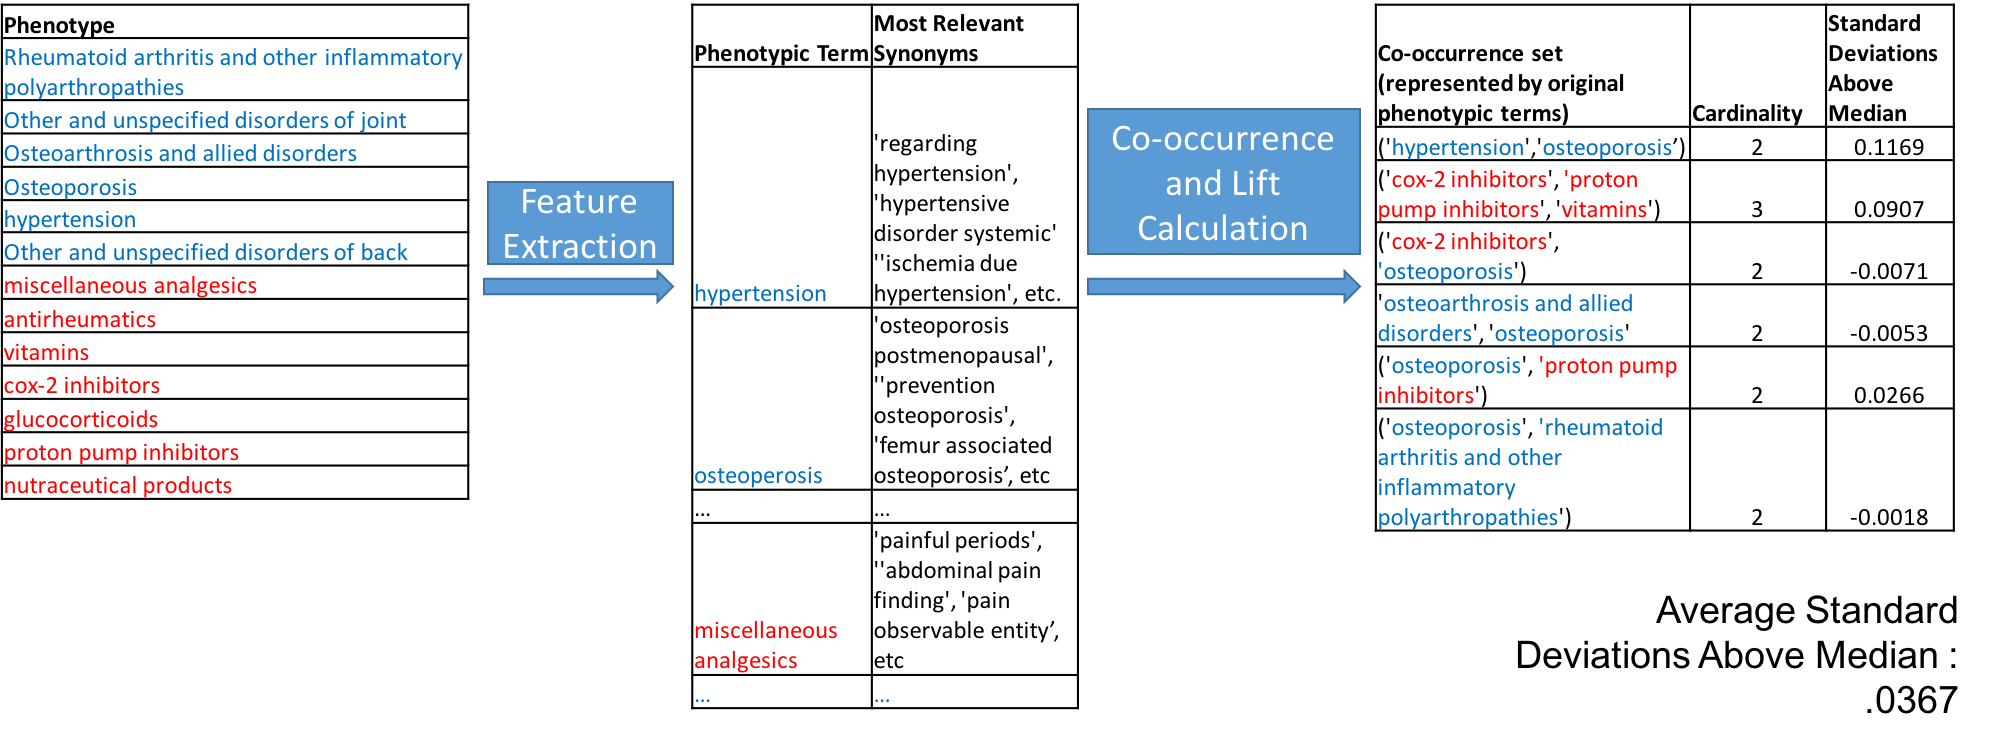
\includegraphics[width=\linewidth]{lift-process-cartoon.png}
\caption{Example of lift calculation process for a phenotype that was found to be significant (i.e., above the threshold of 0.0284)}
\label{fig:lift-process-cartoon}
\end{figure*}


%Table \ref{tab:phenoCard} shows an example of a phenotype with the phenotype cardinality of 6 and a lift of 17. 

We note that the mean and standard deviation of each of these cardinality groups were skewed high, as the max lifts were significantly further from the median than the below-median lifts (Figure \ref{fig:log-lift}). Since the standard deviation is artificially increased by the largest lifts, the normalized above median lifts are still much greater than zero than the below median lifts are below. 
This fact makes it so that a lift threshold is likely to be closer on average to the lift of not significant phenotypes than to significant phenotypes.
Figure \ref{fig:lift-process-cartoon} demonstrates the process of extracting the synonyms for the phenotypic terms, calculating the average standard deviations that a set of phenotypic terms is above the median, and then shows the overall average.
While the middle column only contains a subset of the phenotypic item synonym set, the last column contains all the combinations of phenotypic terms that have non-zero standard deviations (i.e., the co-occurrence is non-zero).
A phenotype is labeled clinically relevant if the average standard deviation of the median is above a chosen threshold.
%Finally, lifts were normalized by the median and standard deviation of the lifts in a phenotype cardinality group.


\section{Empirical Study}\label{empirical}

\subsection{Dataset Description}
Our study uses randomly generated phenotypes, phenotypes curated to represent known significant clinical narratives and the annotated results of candidate phenotypes generated by different unsupervised, high--throughput phenotype generation processes. The first automatic method, Rubik \cite{wang2015rubik},
generated phenotypes from a de--identified EHR dataset from Vanderbilt University Medical Center with 7,744 patients over a five year observation period.
For more details about the pre--processing of the data and phenotype generation, please refer to their paper \cite{wang2015rubik}.
The authors graciously shared the file with 30 computational phenotypes as well as the annotations of the three domain experts.
For each phenotype, each expert assigned one of the following three choices: 1) yes - the phenotype is clinically meaningful, 2) possible - the phenotype is possibly meaningful, and 3) not -- the phenotype is not clinically meaningful.
The second set of candidate phenotypes were generated by Marble \cite{Ho:2014da} using the EHR data of a random subset of 10,000 patients from the \emph{Centers for Medicare and Medicaid Services (CMS) Linkable 2008-2010 Medicare Data Entrepreneurs' Synthetic Public Use File (DE-SynPUF)}, a publicly available dataset with claim records that span 3 years.\footnote{For more information see https://www.cms.gov/Research-Statistics-Data-and-Systems/Downloadable-Public-Use-Files/SynPUFs/DE\_Syn\_PUF.html}
The 50 candidate phenotypes that Marble generated were then annotated by two domain experts in a manner identical to above.
We combined the 30 Rubik-generated candidate phenotypes with the 50 Marble-generated candidate phenotypes and used the resulting set of 80 candidate phenotypes in the co-occurrence experiment.
Of these 80 phenotypes,  the annotators found that approximately 14\% are clinically meaningful, 78\% are possibly significant and 8\% are not clinically meaningful.

In addition to the high--throughput generated phenotypes, we used randomly generated phenotypes and curated phenotypes to establish lower and upper bounds, respectively, for the lift score that measures phenotype significance. The random phenotypes are generated by randomly selecting phenotypic items from a set of 1000+ phenotypic items generated by Marble/Rubik phenotypes not used in this work. The curated phenotypes were constructed by representing clinical narratives described in Epocrates references\footnote{http://www.epocrates.com/} and the AHRQ national guidelines\footnote{http://www.ahrq.gov/professionals/clinicians-providers/guidelines-recommendations/index.html} using phenotypic items. 
%Table \ref{tab:curated-pheno-example} shows a curated phenotype which represents treatment and diseases which disproportionately affect African Americans.

%\begin{table}
%\begin{center}
%\begin{tabular}{l}
%\toprule
%\color{blue}Sickle cell trait \\
%\color{blue}Chest pain, unspecified \\
%\color{blue}Rickets, active \\ 
%\color{blue}diabetes mellitus, type 2 \\ 
%\color{red}miscellaneous antibiotics \\ 
%\color{red}vitamins and minerals \\ 
%\color{red}analgesics \\
%\bottomrule
%\end{tabular}
%\end{center}
%\caption{Example of a curated phenotype representing diseases disproportionately affecting African Americans. Blue entries represent the patient's diagnoses, red entries are medications.}
%\label{tab:curated-pheno-example}
%\end{table}

%\joyce{Describe the dataset you're using and how you came up with significant and random groups}
%\jette{probably describe the phenotype dataset before describing the Empirical study? Maybe lead with the Dataset description and put the following paragraphs in the result subsection }


\begin{figure} [t]
\centering
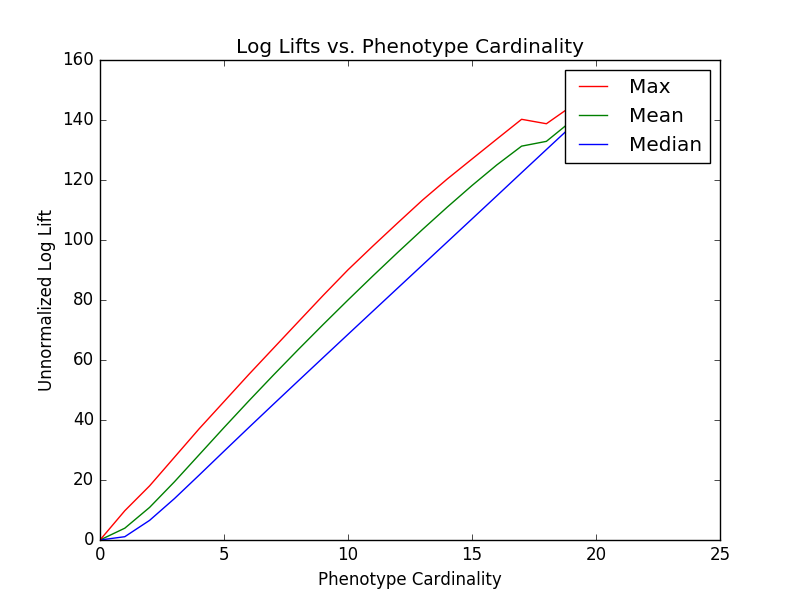
\includegraphics[width=\linewidth]{logLiftsAcrossPhenoCard_MMM_relabeled.png}
\caption{Log Lifts versus Phenotype Cardinality from all Combinations of Phenotypic Items from any Phenotype}
\label{fig:log-lift}
\end{figure}

%\begin{table}
%\begin{center}
%\begin{tabular}{l}
%\toprule
%'Chest pain, unspecified', 'Unspecified chest pain',\\
% 'miscellaneous GI agents','otic preparations',\\
% 'sulfonamides', 'vitamins and minerals' (lift is 17) \\
%\bottomrule
%\end{tabular}
%\end{center}
%\caption{A co-occurrence with 'phenotype cardinality' of 6 and lift of 17}
%\label{tab:phenoCard}
%\end{table}

\subsection{Results}
To determine the optimal size of the phenotypic item synonym set (i.e., the number of ``relevant" n-grams to use), we performed a grid search over the set sizes, the results of which are summarized in Figure \ref{fig:classificationVarNG}.
Figure \ref{fig:classificationVarNG} shows the precision, recall and F1 score for classifying phenotypes to their ``significant" or ``not significant" annotator labels when characterized by different numbers of n-grams. 
The choice of 6 n-grams resulted in classification with the best balance between precision and recall, achieving an F1 score of 0.87 (2 N-grams scored 0.88, but had lower precision).

\begin{figure} [t]
\centering
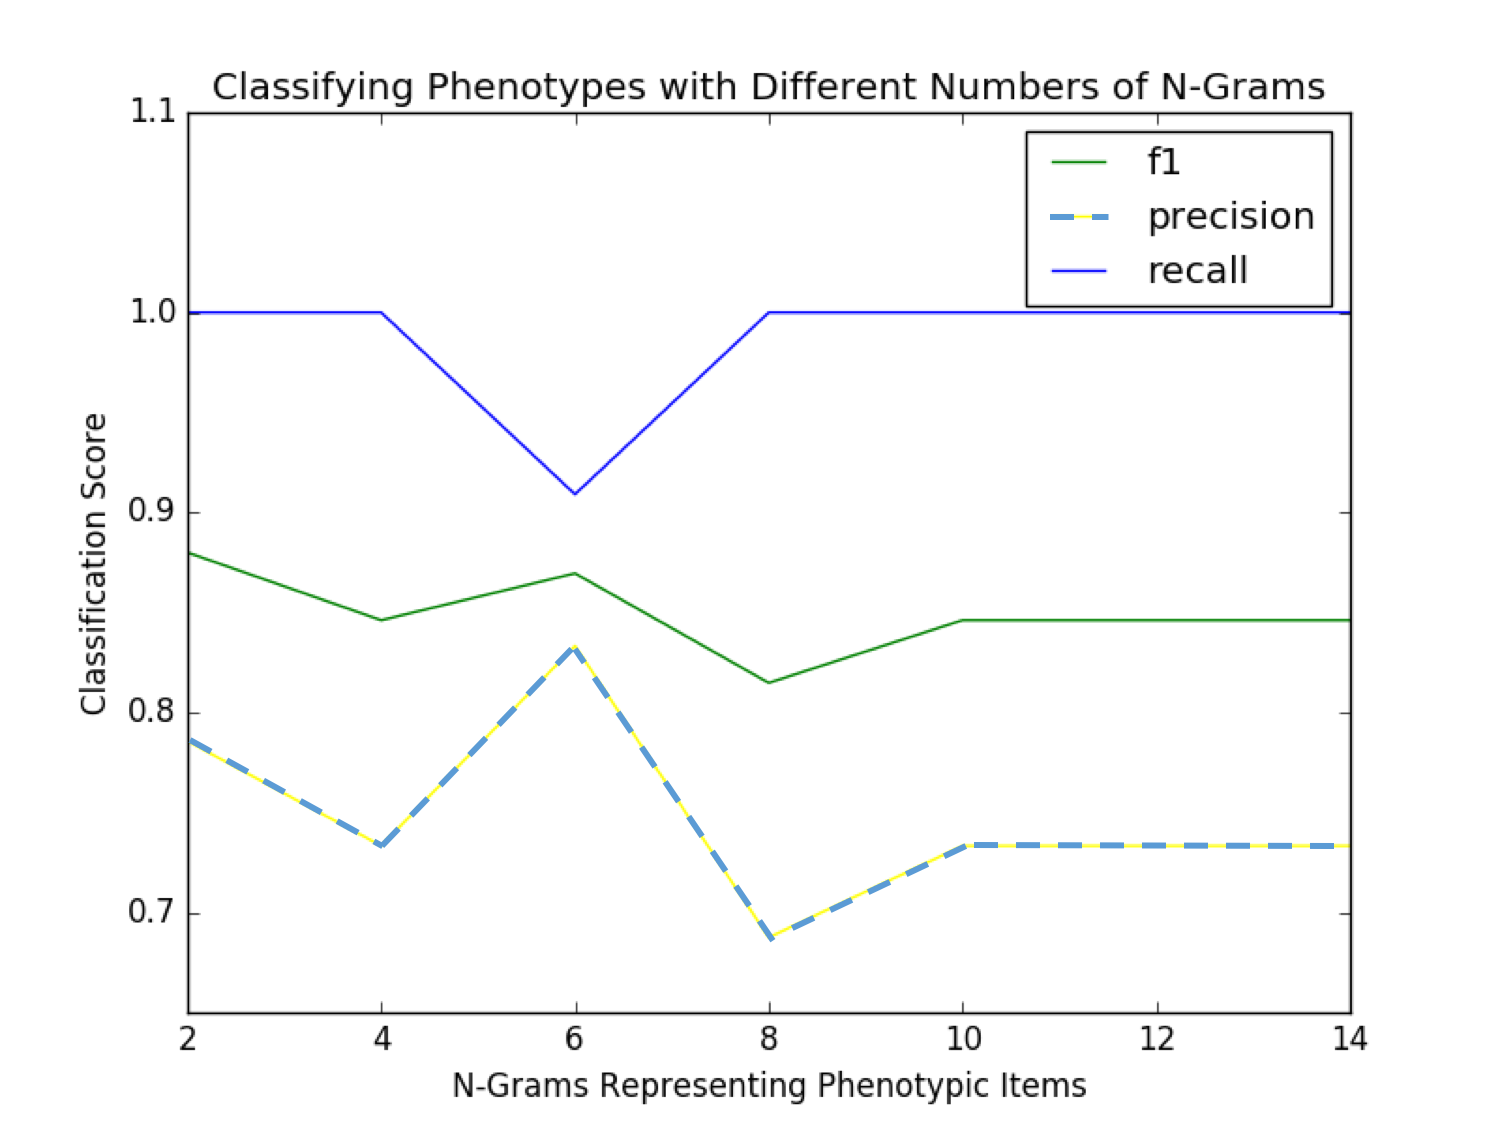
\includegraphics[width=\linewidth] {classificationWithVariableNG_edit.png}
\caption{Classification Scores for Marble/Rubik Phenotypes versus size of Synonym Set}
\label{fig:classificationVarNG}
\end{figure}


\begin{figure} [t]
\centering
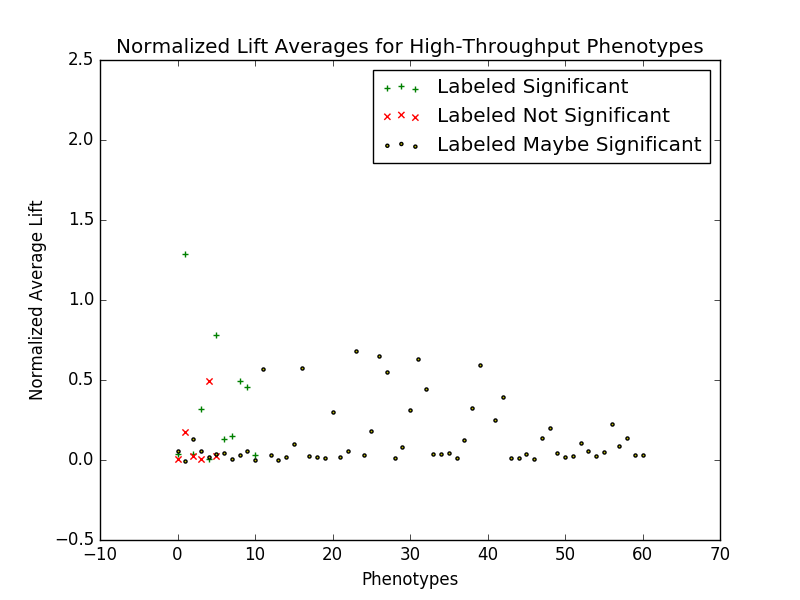
\includegraphics[width=\linewidth]{normalizedLiftAvg_without0s.png}
\caption{Normalized Average Lift of Marble/Rubik Phenotypes}
\label{fig:kho-josh-all}
\end{figure}


\begin{figure} [t]
\centering
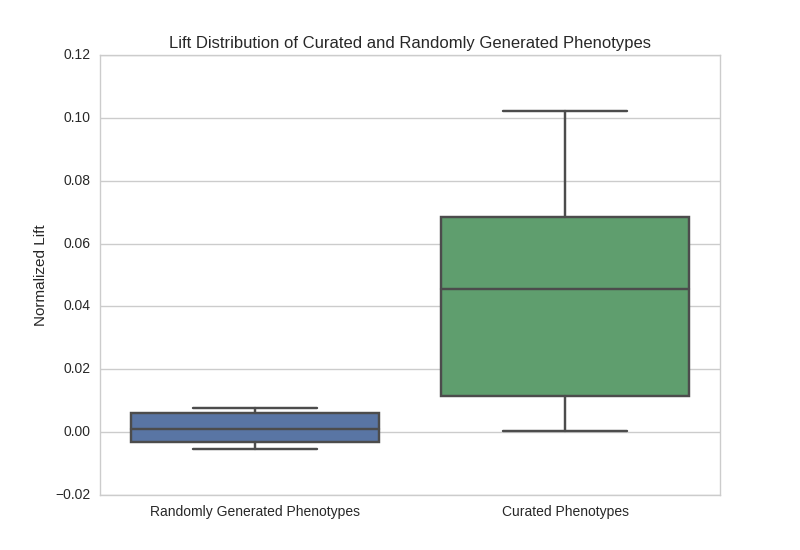
\includegraphics[width=\linewidth] {normalizedLiftAvg_boxplot.png}
\caption{Normalized Average Lift of Curated Phenotypes}
\label{fig:curatedPhenos}
\end{figure}


%\begin{figure} [t]
%\centering
%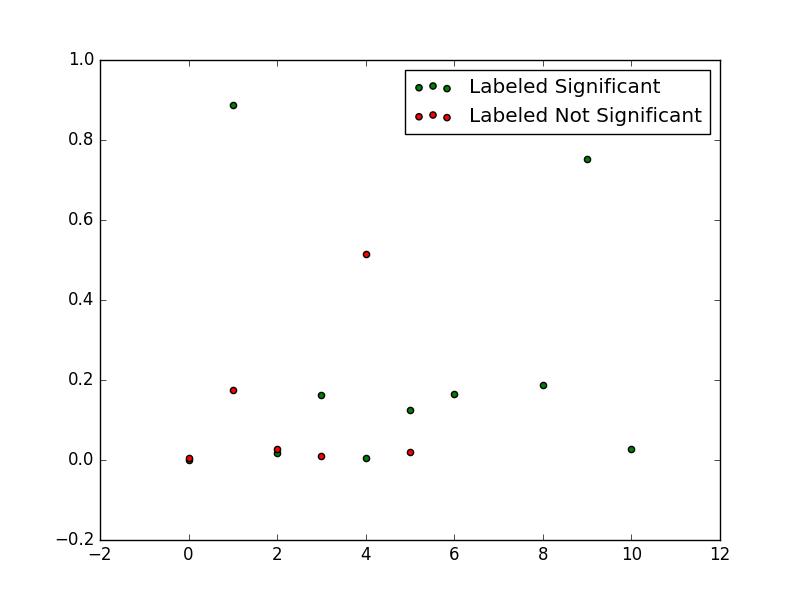
\includegraphics[width=\linewidth]{kho_josh_posneg.png}
%\caption{Normalized Average Lift (Kho, Josh pos neg)}
%\label{fig:kho-josh-posneg}
%\end{figure}



We first examine the normalized lift averages of the randomly generated and curated phenotypes to establish a baseline for the difference between significant and not significant phenotypes. Figure \ref{fig:curatedPhenos} shows the distribution of average lifts for the two groups of phenotypes (represented, again, by a synonym set of 6 N-grams). 
In the majority of cases the normalized lift average of the curated phenotypes is above that of the randomly generated phenotypes. 
By choosing the optimal threshold, we are able to achieve 100\% true negative classification, and 80\% true positive classification, or an F1 score of 0.89. 

Moving on from the separation of random and curated phenotypes, we applied this analysis to real world phenotypes generated by the high-throughput methods. Figure \ref{fig:kho-josh-all} shows the normalized lift average of the phenotypes generated by Marble and Rubik (\cite {Ho:2014jc,Ho:2014da, wang2015rubik}). 
%Figure \ref{fig:kho-josh-all} shows the normalized lift averages for phenotypes labeled as "significant", "maybe significant" and "not significant". 
Again, by determining the optimal lift threshold (determined to be 0.028 by exhaustion), we are able to classify ``significant" and ``not significant" phenotypes with an F1 score of 0.87. 

While we do not perform any classification on the possibly significant groups, we plan to delve into this into the future.
Annotators could use this analysis as evidence to give labels the phenotypes that may be significant.
For example, if an annotator was not sure about the significance, he or she could use the average lift as another piece of information while making the decision.
However, a more thorough analysis of the value of this and whether or not it would bias an annotator must be studied.

We note that while lift thresholding classifies phenotypes with relative success in both high-throughput and curated phenotypes, the method does not provide a universal threshold guaranteed for all phenotypes. In addition, the majority of phenotypes are very close to the optimal threshold. This suggests that further work is needed to improve the predictive value of lift thresholding.

\section{Conclusion}
We have presented an automated method for verifying the significance of phenotype groupings using co-occurrence of diagnoses/medications within the phenotype in a corpus of medical literature. 

By representing phenotypes as a small set of relevant n-grams and calculating the lift of phenotypic item co-occurrences in PubMed, we were able to classify a small set of curated phenotypes with an F1 score of 0.89, and a set of phenotypes generated from EHR tensor data with an F1 score of 0.87. While this ground truth set is small, the method shows promise to provide an objective and automated method of verification for arbitrary phenotype groups. 

Further, since the item co-occurrences are found in natural language, a set of sentences describing the phenotypic item co-occurrence can be reported and synthesized into a human readable explanation for the significance of the phenotype. 
Previous work \cite{neveol2011semi} has shown that annotators produce better annotations in less time when starting from pre-annotated results from automatic tools. 
This implies that in addition to corroborating human annotation, automatic labeling can be used to facilitate the annotation process. 
We wish to examine this more in the future.

Work to further verify and improve this method is merited, as a reasonably high level of classification accuracy was achieved without complex feature selection, or using co-occurrences from the remaining 75\% of available PubMed articles. With these additions, the method could further help improve phenotype annotation quality. 



%
% The following two commands are all you need in the
% initial runs of your .tex file to
% produce the bibliography for the citations in your paper.
% You must have a proper ".bib" file
%  and remember to run:
% latex bibtex latex latex
% to resolve all references
%
% ACM needs 'a single self-contained file'!
%
%APPENDICES are optional
%\balancecolumns


\bibliographystyle{abbrv}
\bibliography{PubMed}  % sigproc.bib is the name of the Bibliography in this case
%\balancecolumns % GM June 2007
% That's all folks!

\end{document}
